%csbd_acl

\documentclass[../../main/main.tex]{subfiles}

\begin{document}
\title{Certified Security by Design (CSBD) \& Access\-Control Logic (ACL)}

%%%%%%%%%%%%%%%%%%%%% Chapter CSBD ACL %%%%%%%%%%%%%%%
\chapter[Certified Security by Design (CSBD) \& Access-Control Logic (ACL)]{Certified Security by Design (CSBD)  \\ \& \\ Access-Control Logic (ACL)} \label{chp:csbdacl}


      %%%%%%%%%%%%%%%%%%% Section CSBD %%%%%%%%%%%%%%%%%%
\section{Certified Security by Design (CSBD)} \label{sec:csbd}
In 1970 The Rand Corporation published a report\cite{defensescienceboard} for the Office of The Director of Defense Research And Engineering.  This report titled, Security Controls For Computer Systems, noted that "Providing satisfactory security controls in a computer system is in itself a system design problem."  NIST 800-160 also highlights the importance of incorporating security into the design phase of the system engineering process.  CSBD focuses on the design phase of systems engineering, applying formal methods to verify that a system satisfies the principle of complete mediation.  

More specifically, CSBD is a method for formally verifying and documenting the security properties of a systems.  It focuses on designing systems that satisfy the principle of complete mediation.  It uses an access-control logic (ACL) to reason about access to security sensitive objects of a system.  It uses computer-aided reasoning such as the Higher Order Logic (HOL) Interactive theorem prover to formally verify and document these security properties.  The outcomes of CSBD applied to a system conform to the guidelines set fourth in NIST 800-160 [verify and discuss this.]

In addition to providing formal proofs that demonstrate satisfiability of complete mediation, CDBD is reproducible.  This means that third parties can also verify the formal proofs. This touches on the heart of formal verification of satisfiability: "don't just take my word for it, prove it for yourself."

\subsection{Formal Verification \& Documentation}\label{ssec:formalverifcationdocumentation}


\subsection{Computer-aided Reasoning}\label{ssec:computeraidedreasoning}

\subsubsection{Higher Order Logic (HOL) Interactive Theorem Prover}\label{ssec:pcompletemediation}



\subsection{The Principle of Complete Mediation}\label{ssec:pcompletemediation}

      %%%%%%%%%%%%%%%%%%% Section ACL %%%%%%%%%%%%%%%%%%%
\section{Access-Control Logic (ACL)} \label{sec:acl}
\subsection{ACL: A Command and Control (C2) Calculus} \label{ssec:aclc2}
This section discusses the access-control logic in sufficient detail to understand the research reported in this master thesis.  The material is adapted from \textit{Access Control, Security, and Trust: A Logical Approach}\cite{ChinOlder}.  For more indepth coverage of the \glsentryshort{acl}, read the text.  Any references to "the text" in this section refer to the aforementioned text book.

\glsentryshort{acl} is a logic for reasoning about access to object.  In the jargon of the day it is a command and control (C2) calculus\footnote{command and control being self-evident and calculus being a method for reasoning}. 

\subsection{Principals}\label{ssec:principals}
Principals should be thought of as actors in the access-control logic.  Principals can make statements or requests.  They can be assigned privileges or authority over objects or actions.  The text defines allowable principals using the identifier \textbf{Princ}:

\begin{center}
\textbf{Princ ::= PName / Princ \& Princ / Princ \textbar  Princ}
\end{center}

This is a recursive definition. \textbf{\textit{PName}} refers to the name of a principal (i.e., Jane, PlatoonLeader, sensor1).  \textbf{\textit{Princ} \& \textit{Princ}} is read "Princ with Princ" or "Princ and Princ" (i.e., Principal1 with Principal2). \textbf{\textit{Princ \textbar  Princ}} is read as "Princ quoting Princ" (i.e., Principal1 quoting Principal2).


\subsection{Propositional Variables, Requests, Authority, and Jurisdiction}\label{ssec:statementsacl}
To reason about access-control and trust, the \glsentryshort{acl} uses propositional variables, requests, authority, and jurisdiction to make statements.

Propositions in logic are assertions that are either true or false.  For example, "I am reading this master thesis" is a proposition because either you are or you are not reading this.  Propositional variables are just place holders for propositions.  For example, "I am reading something", where the propositional variable "something" is what you are reading.

Principals can make requests.  In the \glsentryshort{acl}, principals make requests using the \textit{says} operator.  Requests have the form \textit{P says $\varphi$},  where \textit{P} represents some principal and \textit{$\varphi$} represents some assertion.  For example, \textit{PlatoonLeader says platoonHalt}.  In this example, the Platoon Leader is issuing a command (or request) for the platoon to halt.  

Principals can have authority over assertions.  In the \glsentryshort{acl}, authority is conveyed using the \textit{controls} operator.  Statements of authority have the form \textit{P controls $\varphi$},  where \textit{P} represents some principal and \textit{$\varphi$} represents some assertion.  For example, \textit{PlatoonLeader controls platoonHalt}.  This example states that the Platoon Leader has the authority to issue the command (or request) for the platoon to halt. 

Principals can also have jurisdiction over assertions.  Both authority and jurisdiction use the \textit{controls} operator.  Statements of jurisdiction have the same form as statements of authority.  Statements of authority are typically defined in an organization's policy.  Statements of jurisdiction are statements that are readily believed given the context.  For example, \textit{PresidentOfUS controls (PlatoonLeader controls platoonHalt)}.  In this example, the President of the United States, per the U.S. Constitution, has jurisdiction over the authority invested in the Platoon Leader.  In particular, the President of the United States has the jurisdiction to give the Platoon Leader the authority to command her platoon to halt.

In addition, principals can speak for other principals.  Principals do this using the \textit{speaks for} operator.  The ACL represents the \textit{speaks for} operator with the symbol $\Rightarrow$.  These types of statements have the form \textit{P $\Rightarrow$ Q}, where both \textit{P} and \textit{Q} are principals.  For example, \textit{PlatoonLeader $\Rightarrow$ PresidentOfUS}.  This example states that the Platoon Leader speaks for the President of the United States.  

\subsection{Well-formed Formulas}\label{ssec:wff}
\Glspl{wff} are valid statements in the \glsentryshort{acl}.  All \glsentryshort{ACL} statements must be a \glsentryshort{wff}.  The text book defines the set of \glsentryshortpl{wff} using the identifier \textbf{Form}:

\begin{center}
\textbf{Form} ::= \textbf{PropVar} / $\neg$ \textbf{Form} / (\textbf{Form} $\vee$ \textbf{Form}) / \\ 
	                  (\textbf{Form} $\wedge$ \textbf{Form}) / (\textbf{Form} $\supset$ \textbf{Form}) / (\textbf{Form} $\equiv$ \textbf{Form}) / \\
	                  (\textbf{Princ} $\Rightarrow$ \textbf{Princ}) / (\textbf{Princ} says \textbf{Princ}) / (\textbf{Princ} controls \textbf{Form})
\end{center}

This is a recursive definition.  \textbf{\textit{PropVar}} is a propositional variable.  The symbols $\neg$, $\vee$, $\wedge$, $\subset$, and $\equiv$ are the standard set and logical symbols.  They represent "not", "or", "and", "subset", and "equivalence", respectively.  This master thesis primarily reasons with statements (\glsentryshortpl{wff}) of the form \textit{\textbf{Princ} says \textbf{Princ}} and \textit{\textbf{Princ} controls \textbf{Form}}.

\subsection{Kripke Structure}\label{ssec:kripke}
A Kripke structure deals with three things: worlds, propositions, and principals.  The worlds can be thought of as possible states or configurations of some system.  Propositions are just statements that are either true or false.  And, principals are just actors.  A Kripke structure $\mathcal{M}$ = $\langle \textit{W}, \textit{I}, \textit{J} \rangle $  is defined as a three-tuple consisting of a set of worlds \textit{W}, a function \textit{I} that maps propositions to worlds, and a functions \textit{J} that maps principals to relations on worlds.  A more formal definition is definition 2.1 in the text:

\begin{itemize}
\item \textit{W is a nonempty set, whose elements are called worlds.}
\item \textit{$I: \mathbf{PropVar} \rightarrow \mathcal{P}(W)$ is an interpretation function that maps each propositional variable to a set of worlds.}
\item \textit{$J: \mathbf{PName} \rightarrow \mathcal{P}((W \times W)$ is a function that maps each principal name to a relation on worlds.}
\end{itemize}

\begin{figure}[h]
\centering
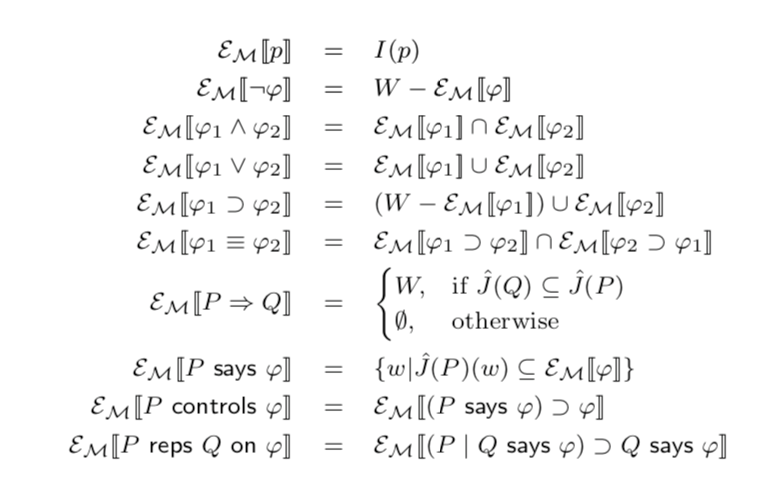
\includegraphics{../figures/kripkesemantics}
\caption{\label{kripkesemantics} Kripke semantics. Image taken from \textit{Access Control, Security, and Trust: A Logical Approach}\cite{ChinOlder}}
\end{figure}


\subsubsection{satisies}\label{sssec:satisfies}
\subsubsection{soundness}\label{sssec:soundness}

\subsection{Inference Rules}\label{ssec:inferencerules}
The inference rules for the \gls{acl} are shown in figure \ref{inferencerules}.  All the inference rules are sound.  Details of proofs of soundness can be found in \textit{Access Control, Security, and Trust: A Logical Approach}\cite{ChinOlder}.

\begin{figure}[h]
\centering
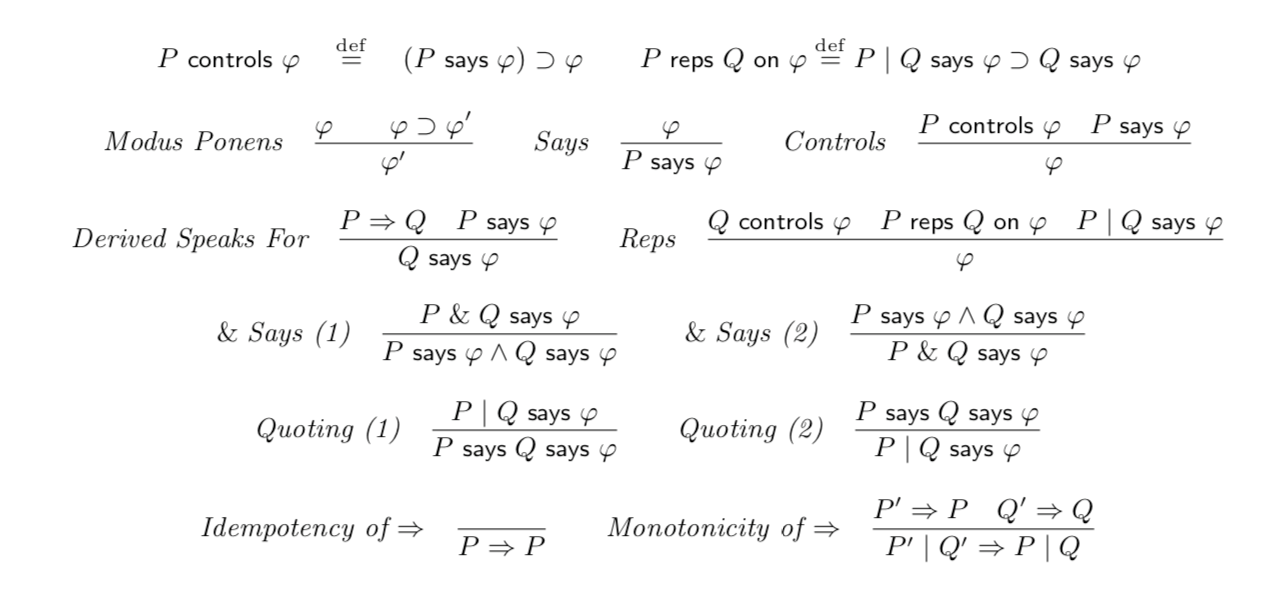
\includegraphics[width=\textwidth]{../figures/inferencerules}
\caption{\label{inferencerules}The \gls{acl} inference rules. Image taken from \textit{Access Control, Security, and Trust: A Logical Approach}\cite{ChinOlder}}
\end{figure}

\subsection{Complete mediation}\label{ssec:aclcompletemediation}
Fundamental to this work is the concept of complete mediation (discussed in section \ref{ssec:pcompletemediation}).  In the \glsunset{acl}\gls{acl}, this means that each principal must be authenticated and authorized on each request.   ACL does this primarily by the \textit{Controls} inference rule in figure \ref{inferencerules} and shown again here in figure \ref{ControlsInferenceRule}. 

\begin{figure}[h]
\centering
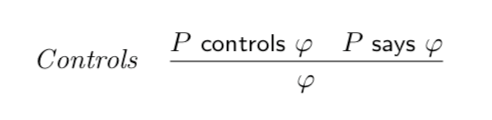
\includegraphics{../figures/ControlsInferenceRule}
\caption{\label{ControlsInferenceRule}The \textit{Controls} inference rule. Image taken from \textit{Access Control, Security, and Trust: A Logical Approach}\cite{ChinOlder}}
\end{figure}

ACL refers to the left statement as an authorization\footnote{or a \textit{control} in the C2 calculus}.  The principal P controls (is authorized on) some action $\varphi$. ACL refers to the right statement in this inference rule as a request \footnote{or a \textit{command} in the C2 calculus}.  The principal P requests some action $\varphi$. The conjunction of the authorization and the request of P on $\varphi$ results in the action $\varphi$.  That is, if \textit{P controls $\varphi$} and\textit{ P says $\varphi$} then $\varphi$  is true.  


The \textit{Reps} rule also demonstrates complete mediation.  It follows a similar logic.  However, the \textit{Reps} rule is not used in this master thesis.

      %%%%%%%%%%%%%%%%%%% Section ACL in HOL %%%%%%%%%%%%%%%
\section{ACL in HOL} \label{sec:aclinhol}
The equivalence of the \gls{acl} formulas implemented in HOL are shown in figure \ref{aclformulasHOL}.

\begin{figure}[h]
\centering
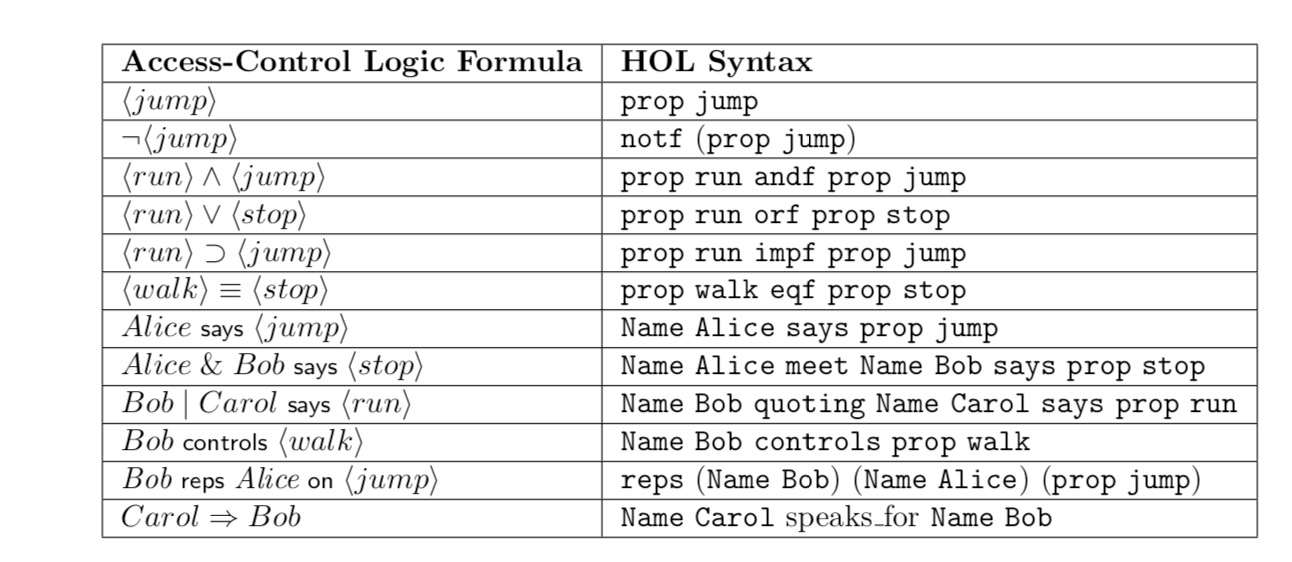
\includegraphics[width=\textwidth]{../figures/aclformulasHOL}
\caption{\label{aclformulasHOL}The \gls{acl} formulas in HOL.  Image taken from \textit{Access Control, Security, and Trust: A Logical Approach}\cite{ChinOlder}}
\end{figure}

Using this syntax, an ACL request of the form \textit{P says \textphi} would have the form
\centerline{ \textit{Name P says prop \textphi}}


\subsection{Complete Mediation}
\subsection{satList}


\end{document}
